\chapter{Results}

%	<Paragraph> Overview of results
This chapter provides results of the $k$-{\sc Sat} execution test from the previous chapter.  We consider the results of the test and provide analysis of the algorithm metrics.  

Design considerations for a physical molecular computation environment extend the algorithm test results.  Selection of a molecular {\sc Satisfiability} algorithm considers the simulation results and practical implementation techniques.

	\section{Algorithm metric comparison}
	
%		<Paragraph> Summary of measured metrics
This section provides results from the simulation.  We provide the analysis for the molecular operations.  These include counts of append, extract, mix, purify, splice, and split.  Presentation of actual computation time and required memory for the solution representation allow for comparison of algorithms.

\FloatBarrier
		
%\subsection{Append}

%%%%%%%%%%%%%%%%%%%%%%%%%%%%%%%%%
\begin{figure}[htdp]

\reversemarginpar{
\textbf{Append} is an operation that concatenates molecules. \\

The Distribution algorithm is exponential in the number of appends.  The operation count for append depends on the parsing order of the \textsf{CNF} expression.\\

Lipton's and Ogihara-Ray's algorithms use a fixed amount of appends.  This depends on the number of variables and clauses present in the \textsf{CNF} expression.
}

\begin{center}

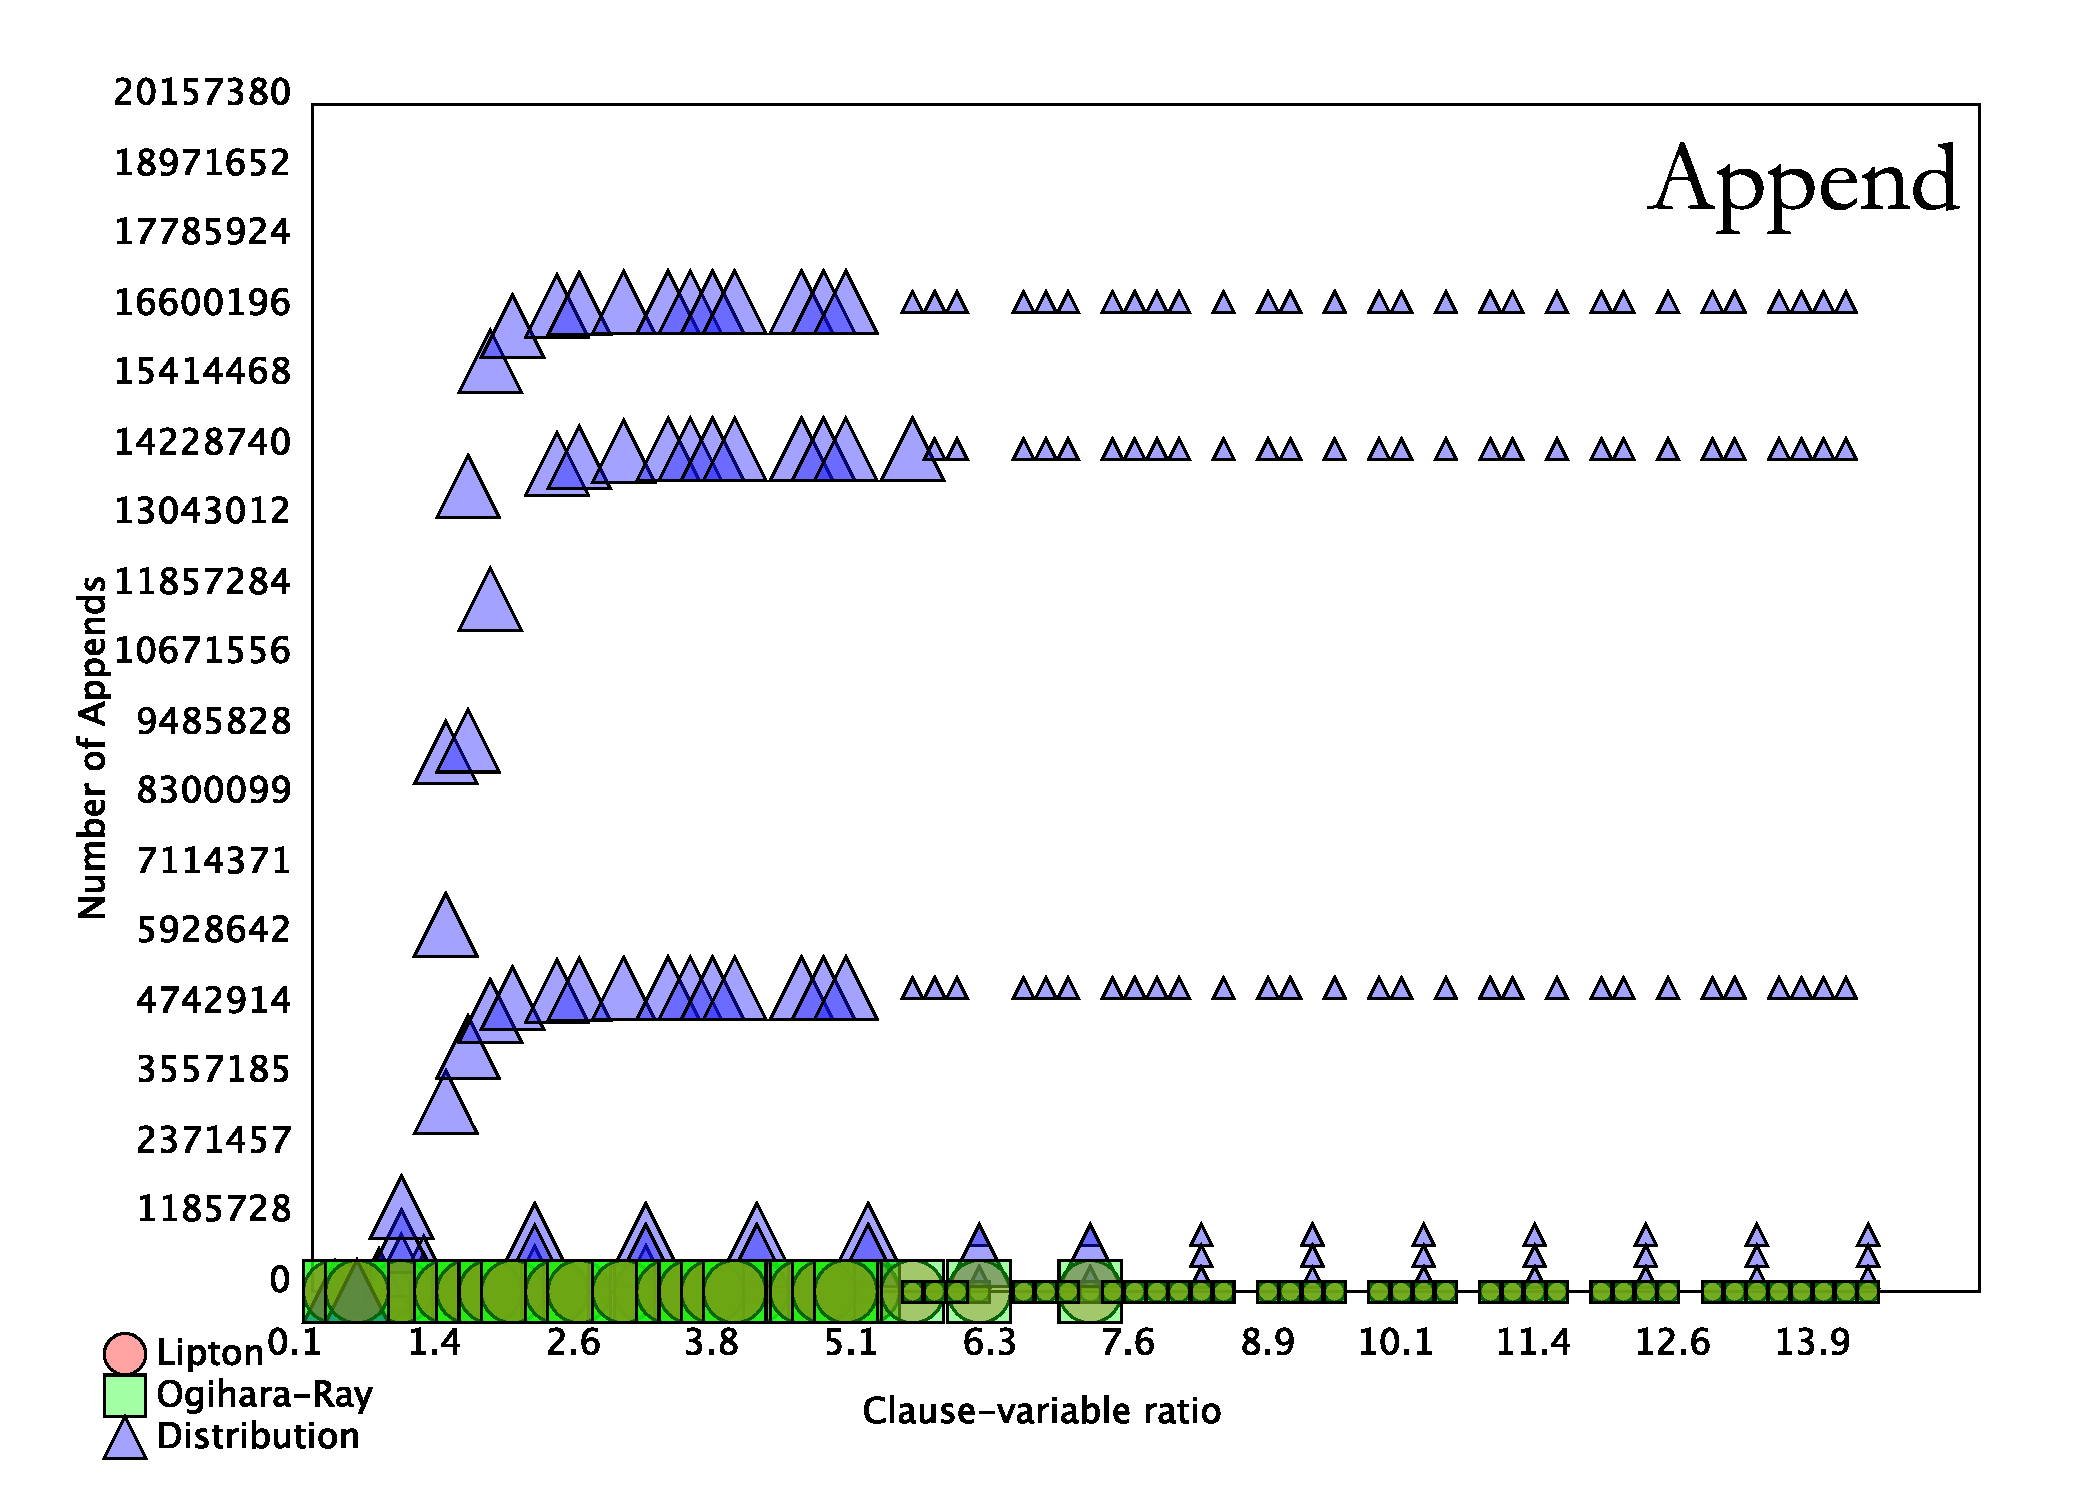
\includegraphics[width=1.1\textwidth]{./figures/metricOutput/Append.pdf}

\caption{Clause to variable ratio $\alpha$ vs. Number of appends }
\label{appendFig}
\end{center}
\end{figure}
%%%%%%%%%%%%%%%%%%%%%%%%%%%%%%%%%

\FloatBarrier
			
%\subsection{Extract}
%%%%%%%%%%%%%%%%%%%%%%%%%%%%%%%%%
\begin{figure}[htdp]

\reversemarginpar{

\textbf{Extract} is an operation that filters strings.\\

Ogihara-Ray's algorithm requires the greatest amount of extracts.  Lipton's algorithm is linear on $\alpha$ and varies a constant amount from Ogihara-Ray's algorithm.\\

The Distribution algorithm does not require extract.

}

\begin{center}

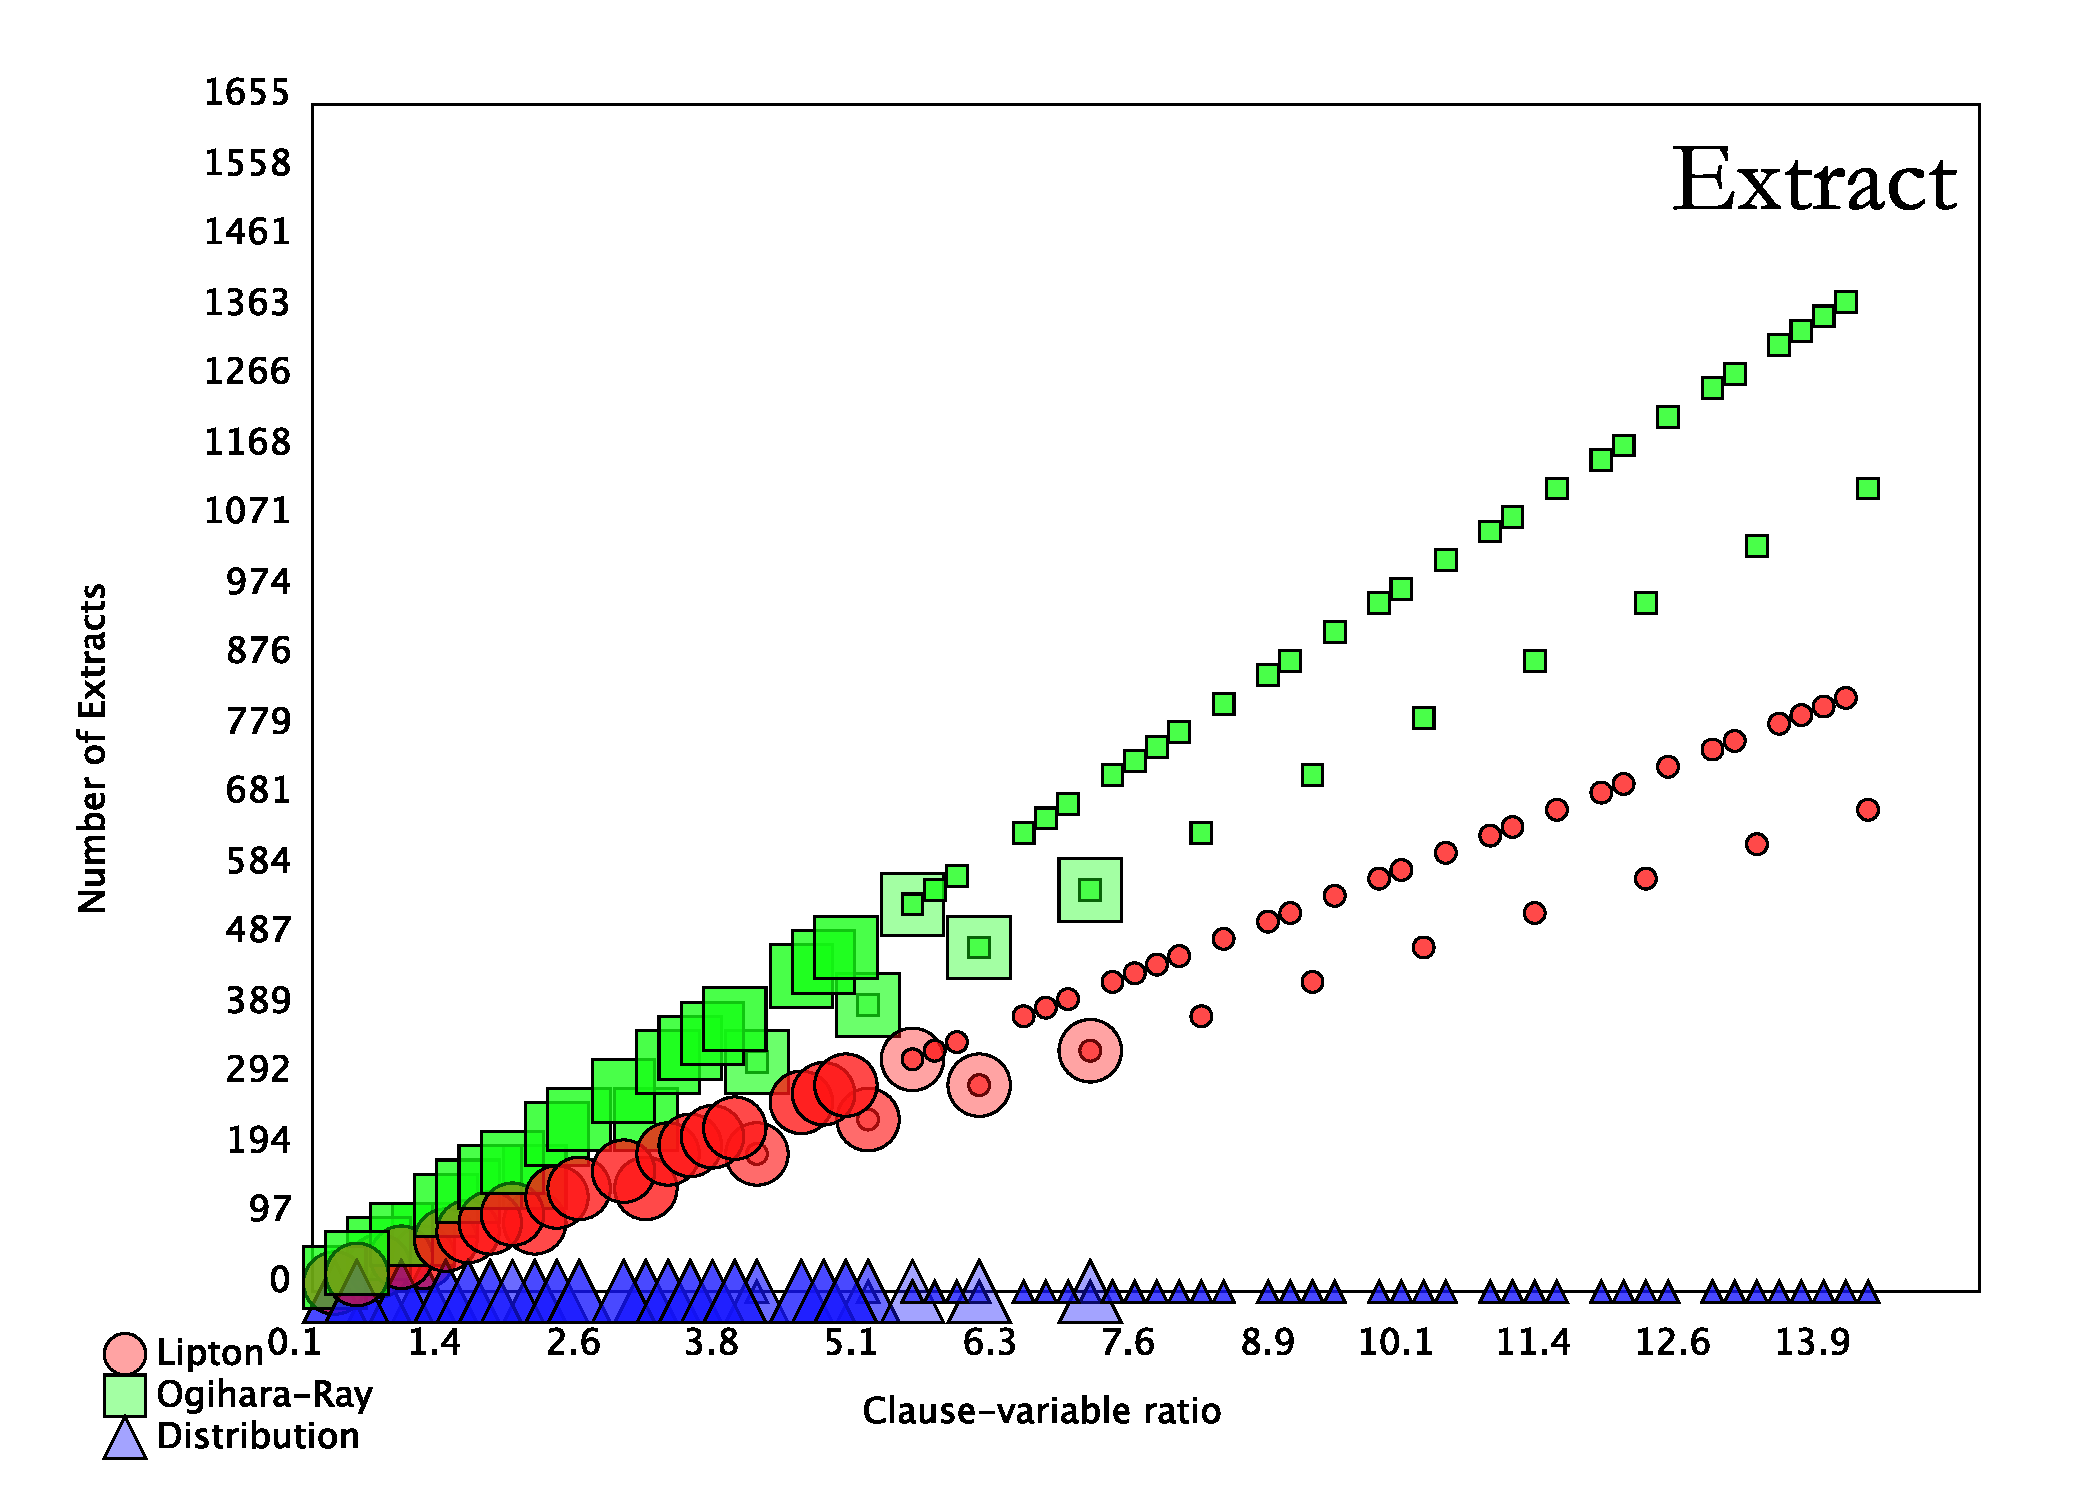
\includegraphics[width=1.1\textwidth]{./figures/metricOutput/Extract.pdf}

\caption{Clause to variable ratio $\alpha$ vs. Number of extracts }
\label{extractFig}
\end{center}
\end{figure}
%%%%%%%%%%%%%%%%%%%%%%%%%%%%%%%%%
\FloatBarrier			
			
%\subsection{Mix}
%%%%%%%%%%%%%%%%%%%%%%%%%%%%%%%%%
\begin{figure}[htdp]

\reversemarginpar{
\textbf{Mix} is an operation that combines two tubes.\\

Lipton's algorithm requires a linear amount of mixes on $\alpha$.  The Distribution algorithm also requires a linear number of mixes, varying by a constant factor from Lipton's algorithm.\\

Ogihara-Ray's algorithm requires a constant amount of mixes on $\alpha$.
}

\begin{center}

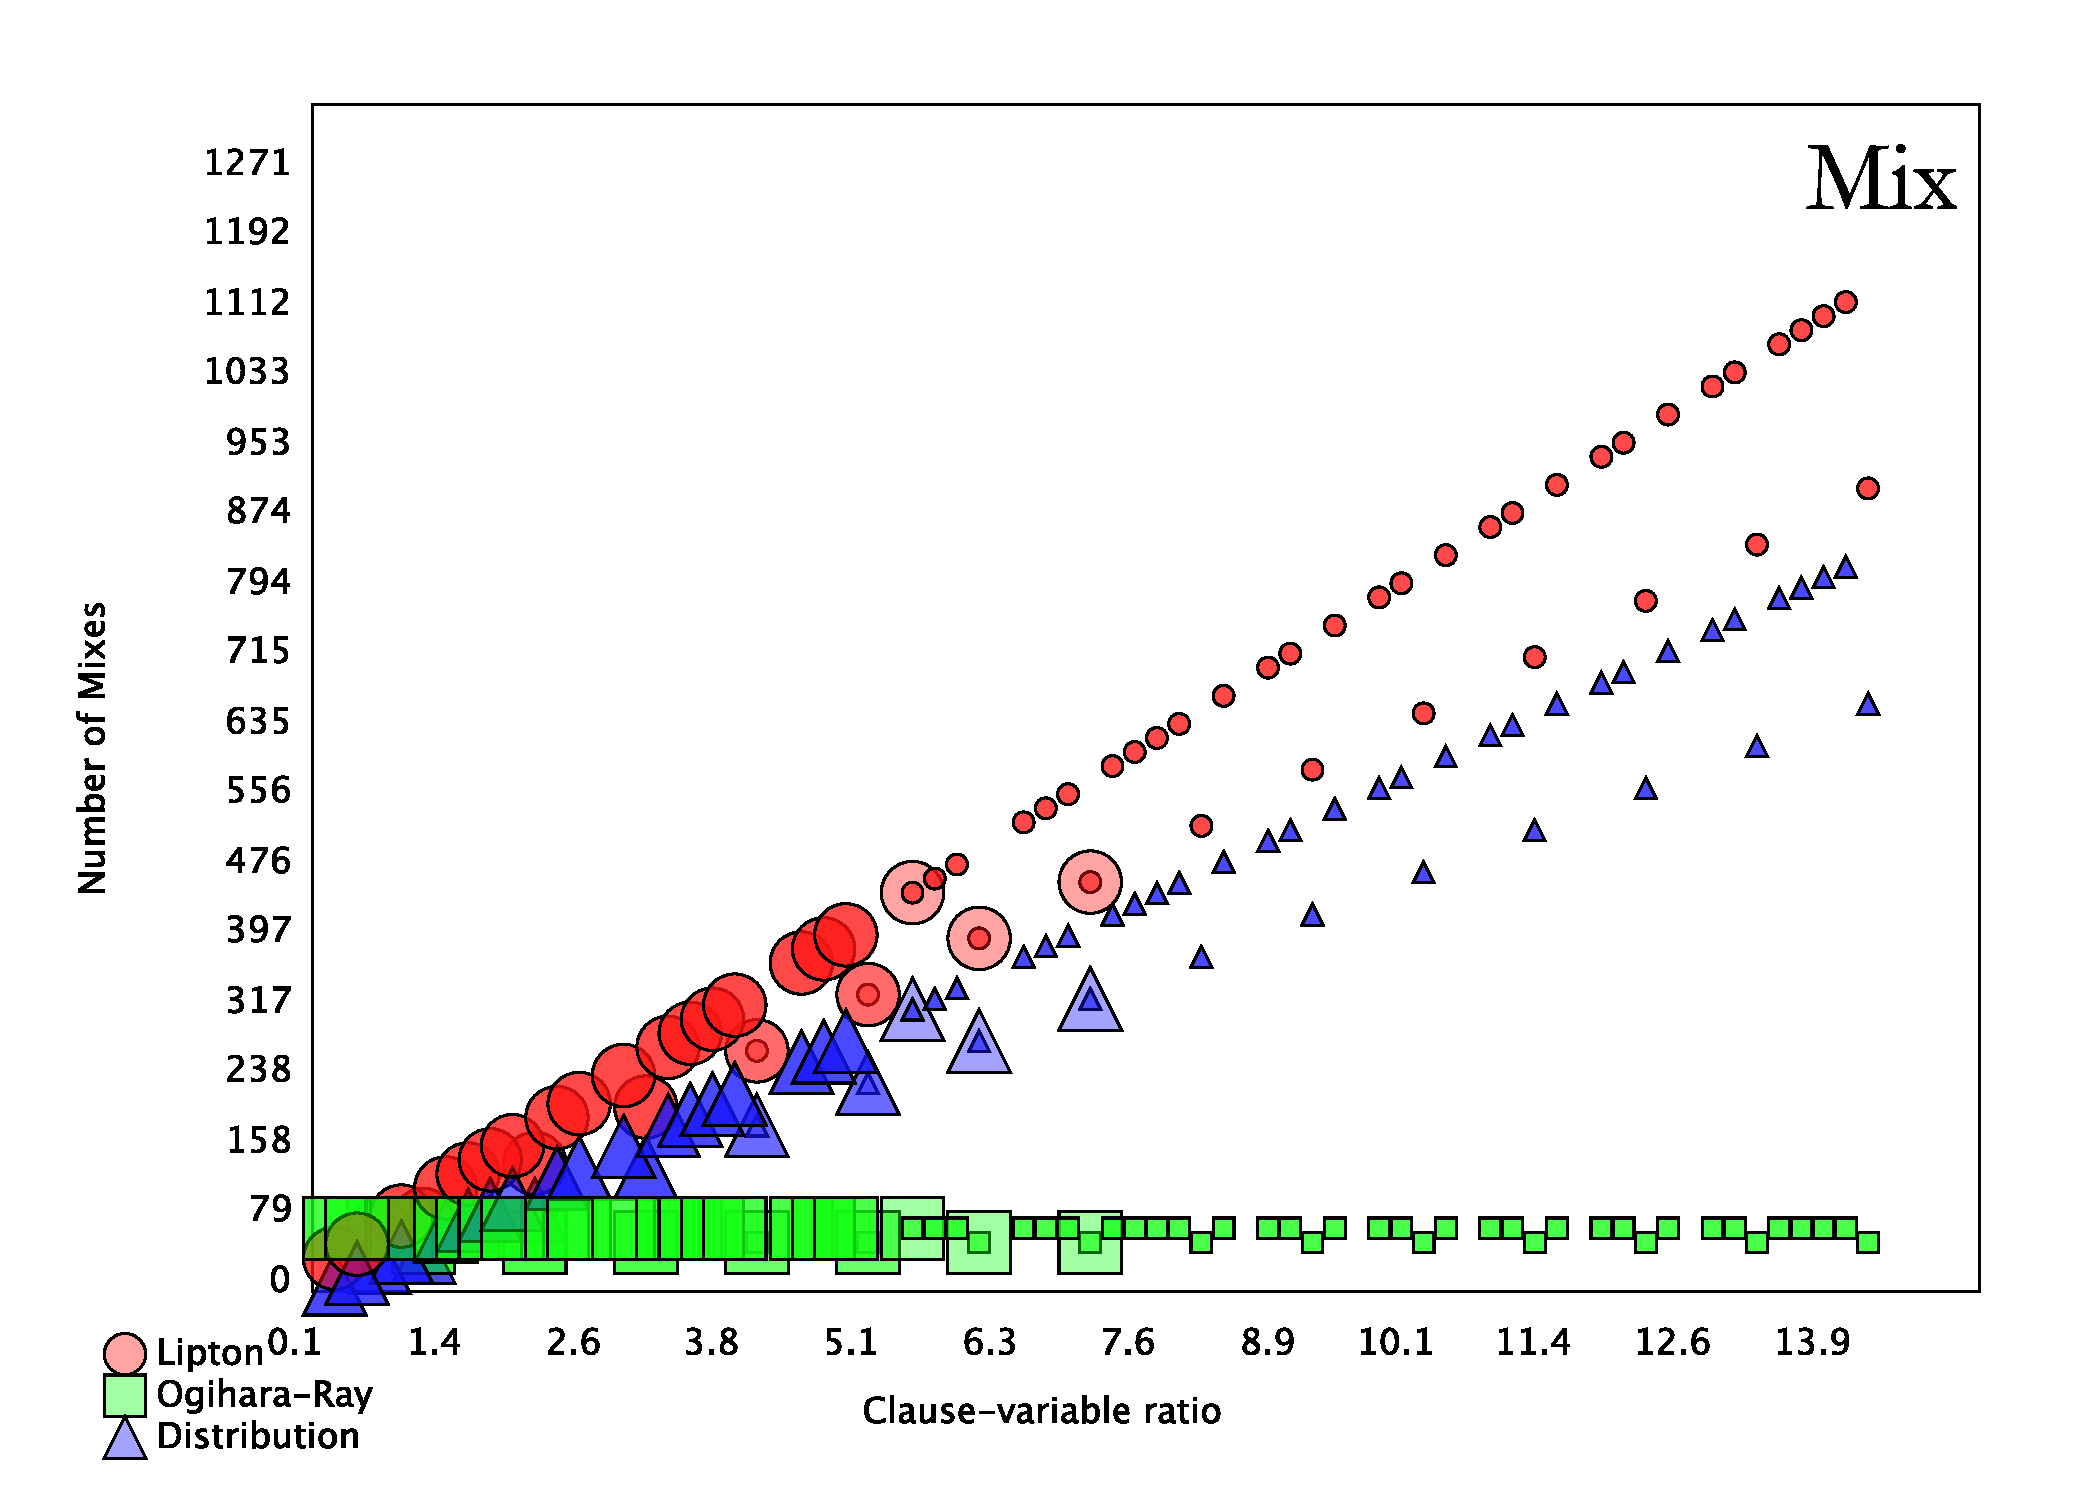
\includegraphics[width=1.1\textwidth]{./figures/metricOutput/Mix.pdf}

\caption{Clause to variable ratio $\alpha$ vs. Number of mixes }
\label{mixFig}
\end{center}
\end{figure}
%%%%%%%%%%%%%%%%%%%%%%%%%%%%%%%%%
\FloatBarrier

%\subsection{Purify}
%%%%%%%%%%%%%%%%%%%%%%%%%%%%%%%%%
\begin{figure}[htdp]

\reversemarginpar{
\textbf{Purify} is an operation that ensures equal portions of each independent string.\\

All three algorithms operate with a  linear  number of purifications on $\alpha$.  Ogihara-Ray's algorithm requires the greatest amount of purifications.  The purifications vary by a constant amount when compared with Lipton's and the Distribution algorithms.

 }

\begin{center}

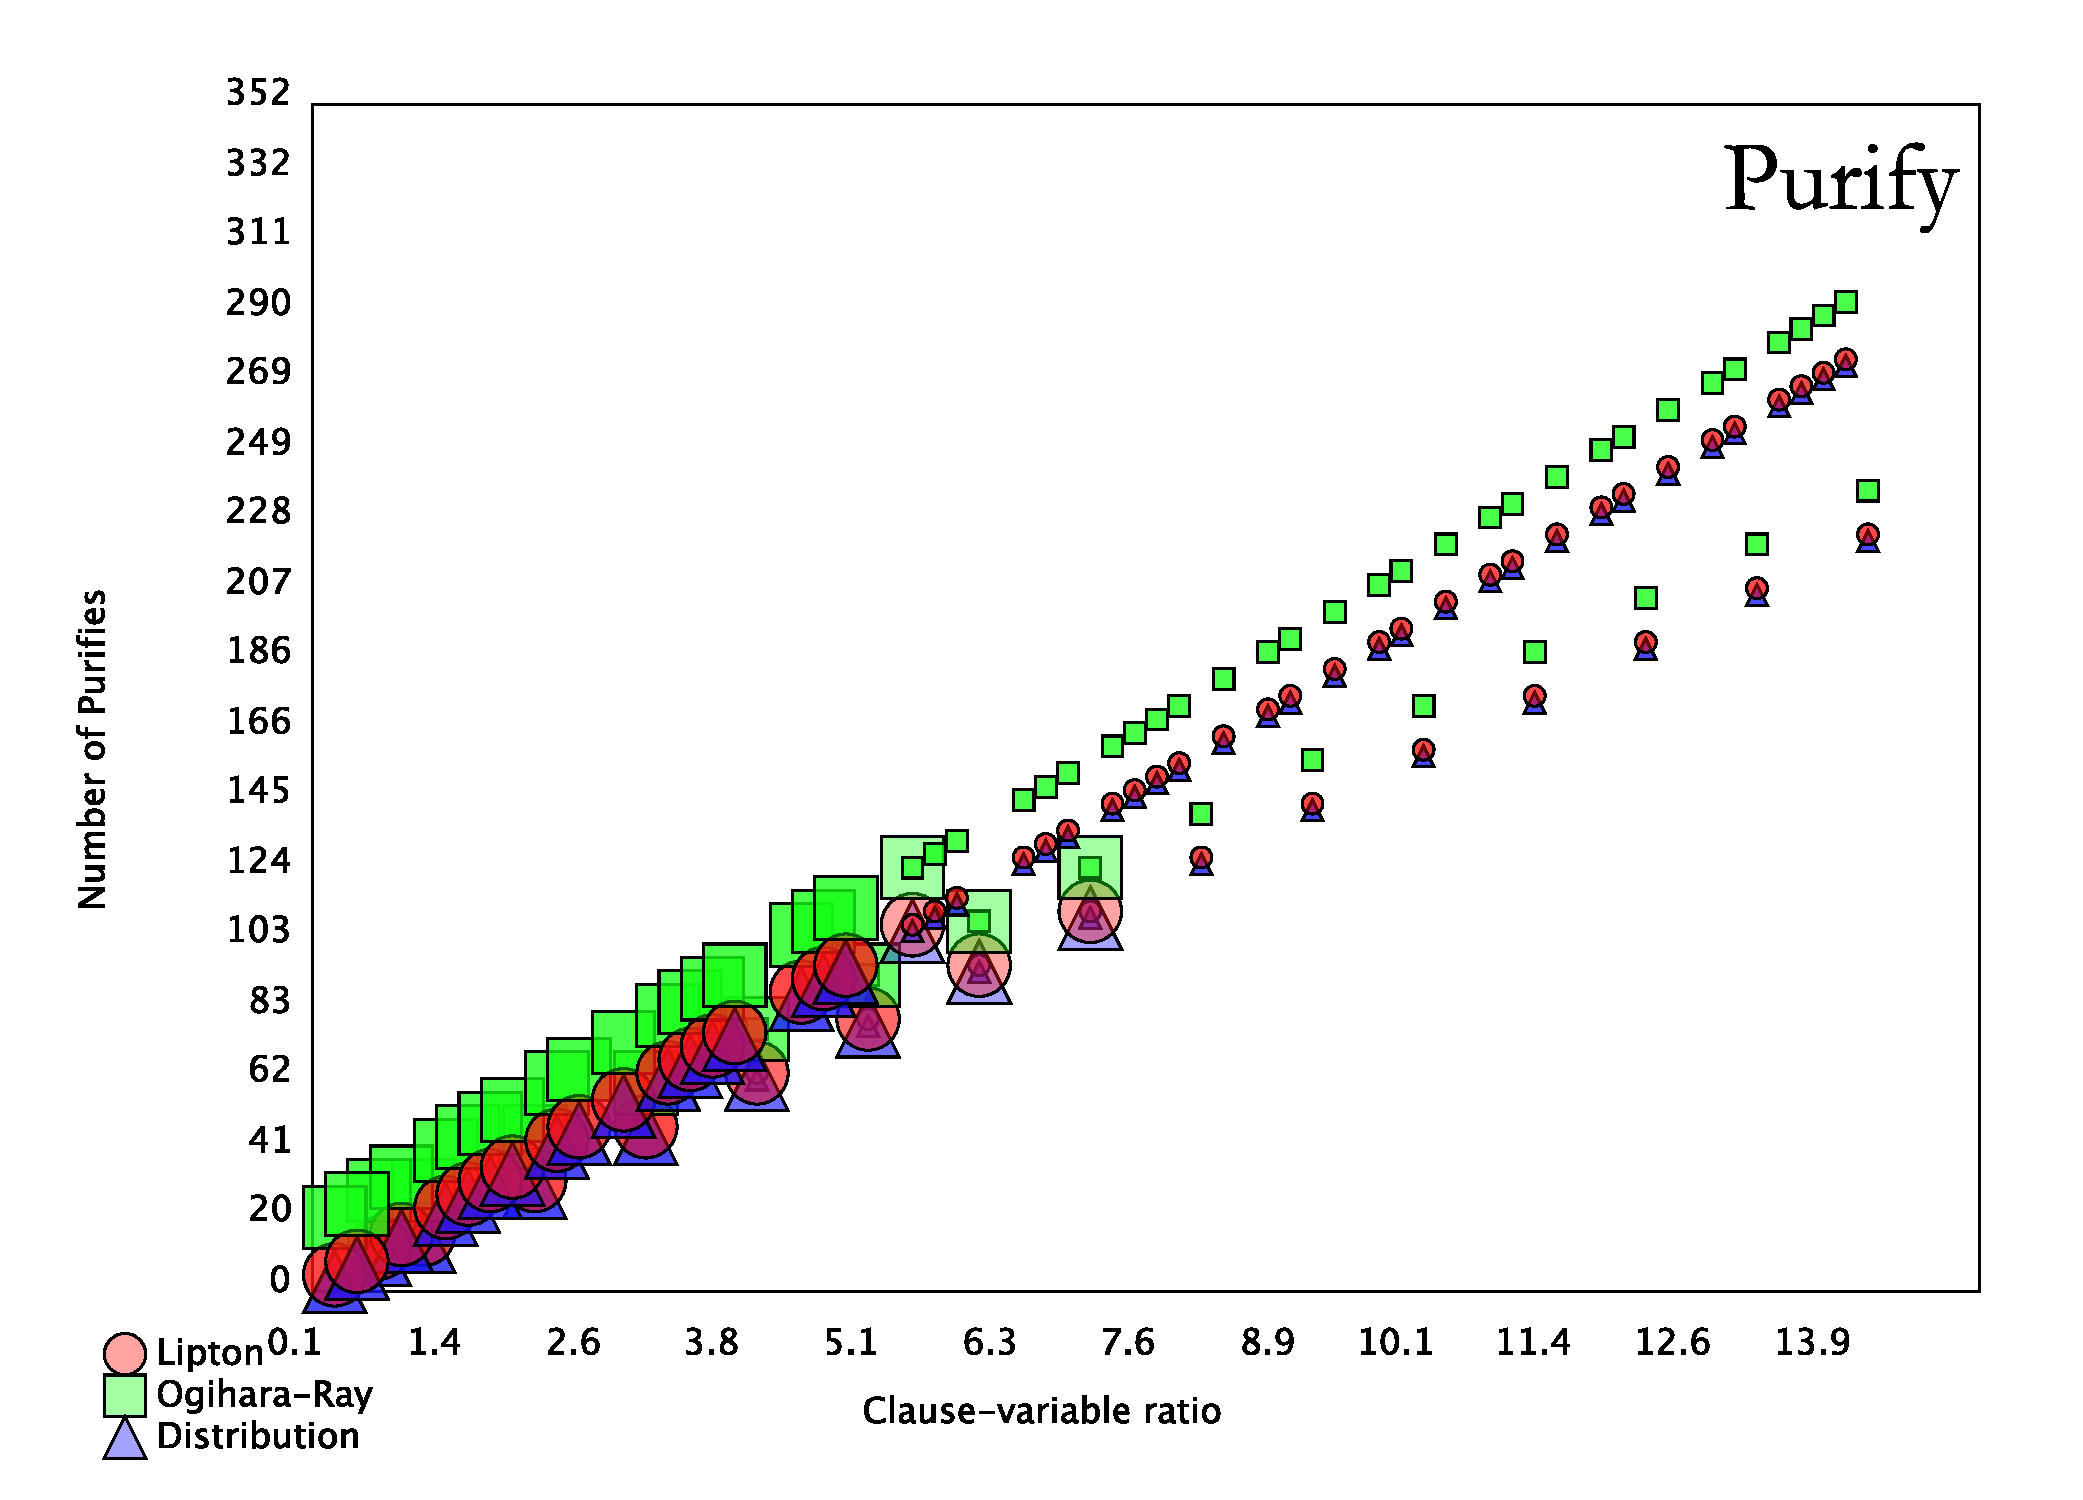
\includegraphics[width=1.1\textwidth]{./figures/metricOutput/Purify.pdf}

\caption{Clause to variable ratio $\alpha$ vs. Number of purifies }
\label{purifyFig}
\end{center}
\end{figure}
%%%%%%%%%%%%%%%%%%%%%%%%%%%%%%%%%
\FloatBarrier

%\subsection{Splice}
%%%%%%%%%%%%%%%%%%%%%%%%%%%%%%%%%
\begin{figure}[htdp]

\reversemarginpar{
\textbf{Splice} is an operation that inserts a string at a targeted location.\\

The Distribution algorithm is exponential in the number of splices.  The number of splices depends on the parsing order of the \textsf{CNF} expression.  Each split requires reassembly, accomplished with two appends.  Figure \ref{appendFig} shows the number of appends.\\

Lipton's and Ogihara-Ray's algorithms do not require splice the splice operator.
}

\begin{center}

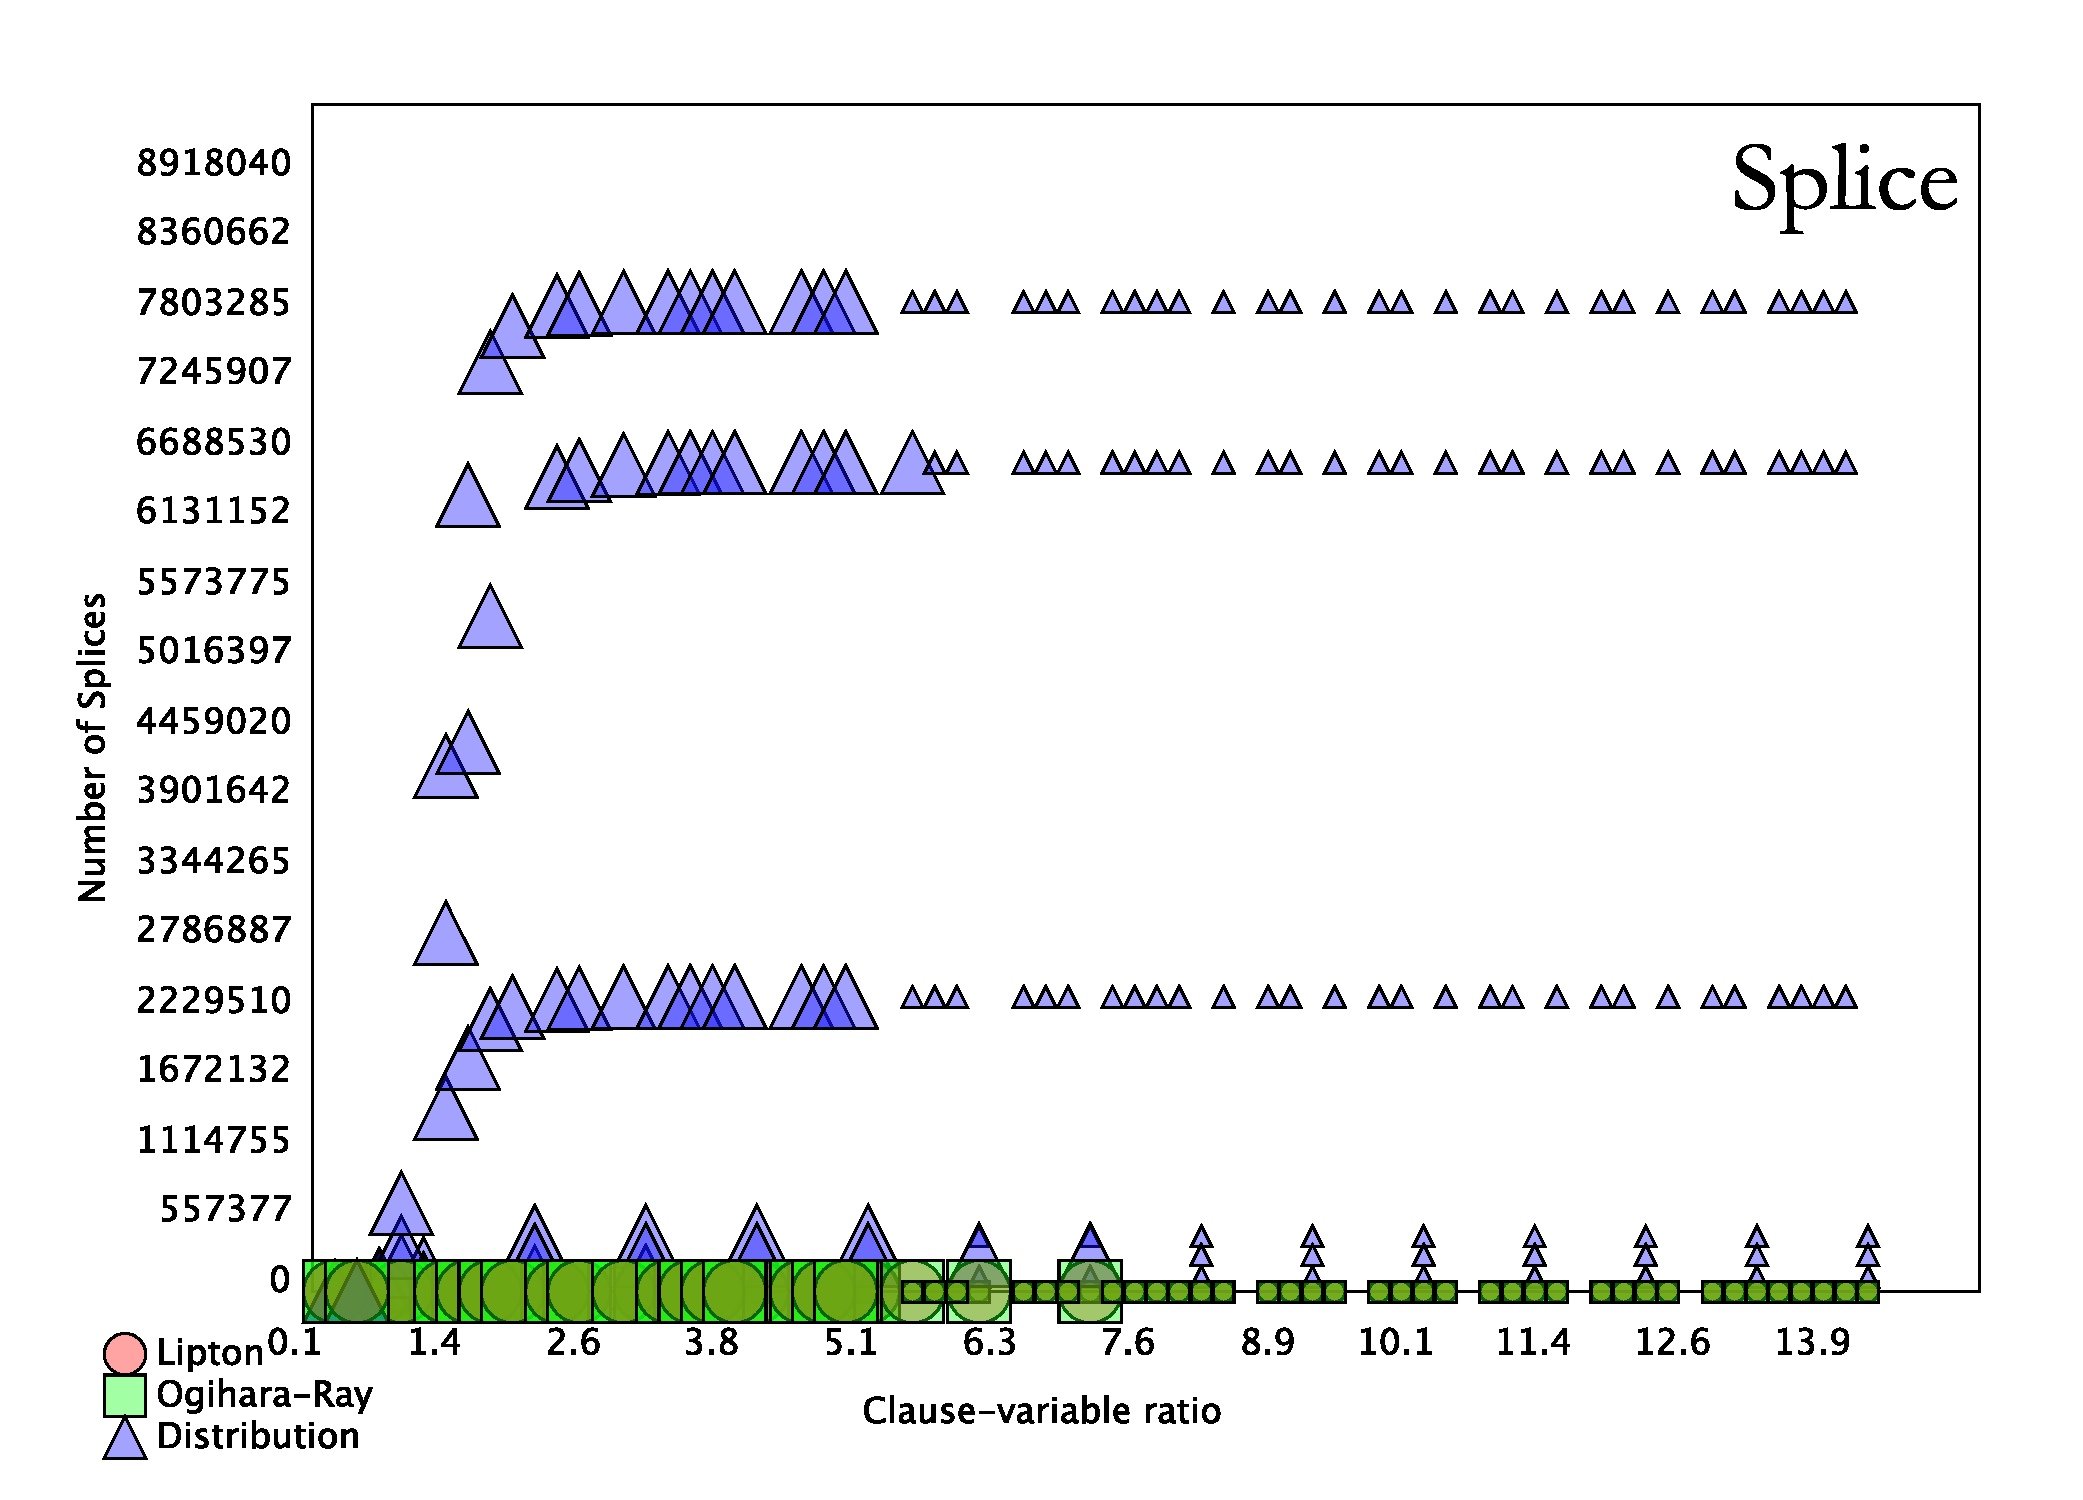
\includegraphics[width=1.1\textwidth]{./figures/metricOutput/Splice.pdf}

\caption{Clause to variable ratio $\alpha$ vs. Number of splices }
\label{spliceFig}
\end{center}
\end{figure}
%%%%%%%%%%%%%%%%%%%%%%%%%%%%%%%%%
\FloatBarrier

%\subsection{Split}
%%%%%%%%%%%%%%%%%%%%%%%%%%%%%%%%%
\begin{figure}[htdp]

\reversemarginpar{

\textbf{Split} is an operation that portions a tube into two exact copes.\\

Distribution requires a linear number of splits.\\

Lipton's and Ogihara-Ray's algorithms are constant in splits based the number of variables.
 }

\begin{center}

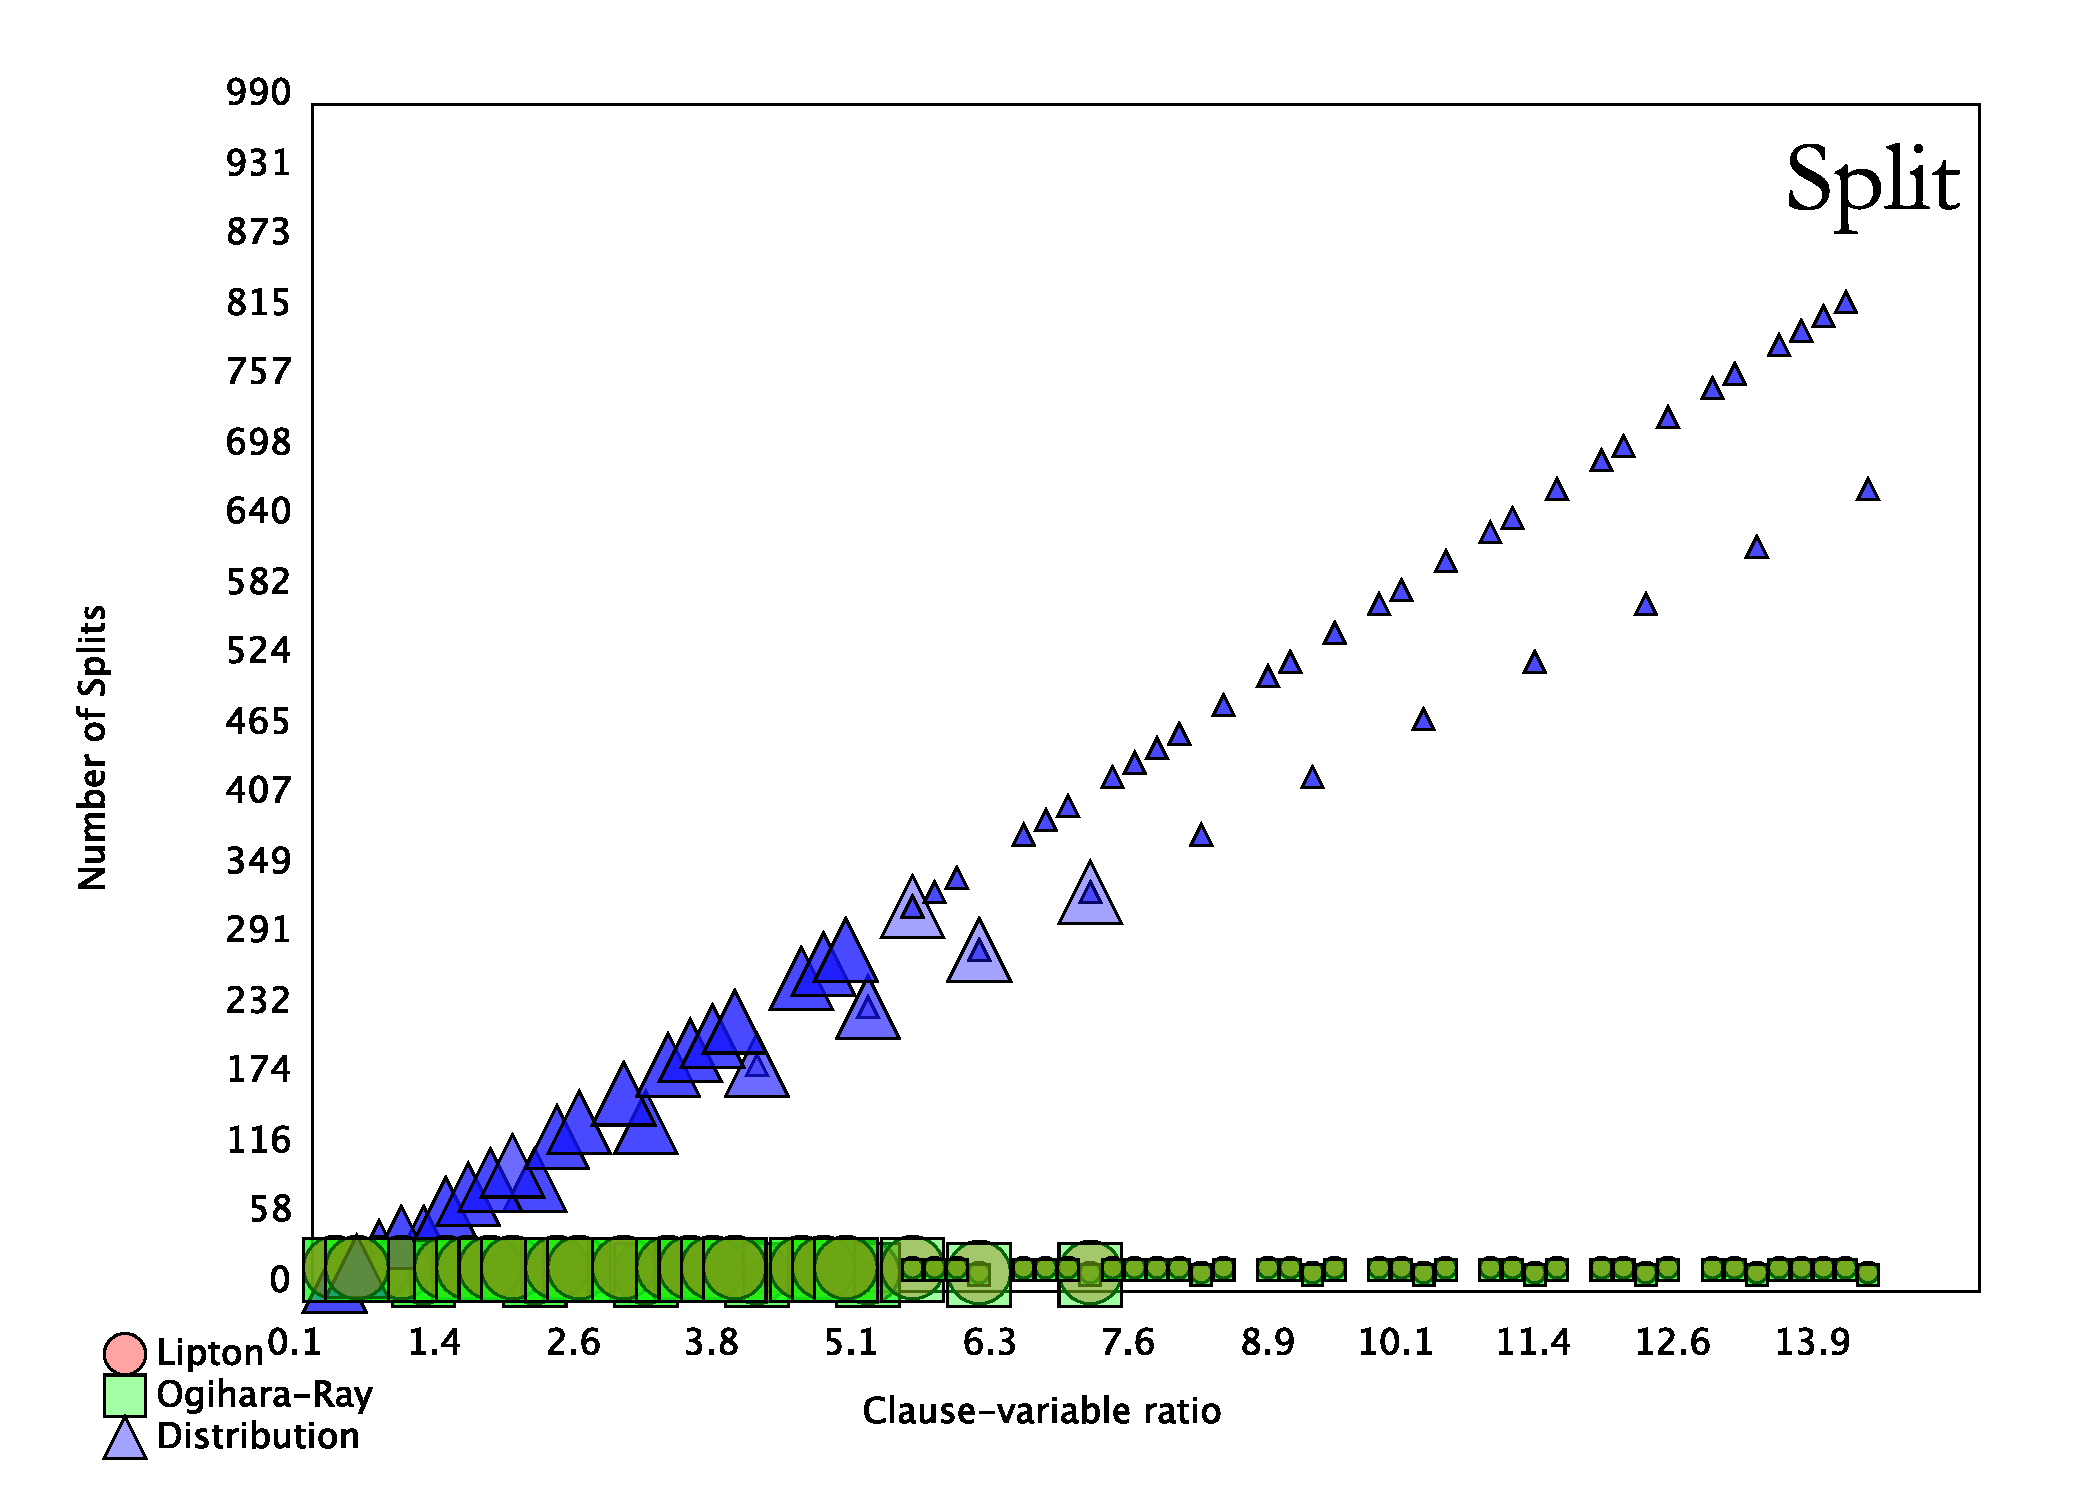
\includegraphics[width=1.1\textwidth]{./figures/metricOutput/Split.pdf}

\caption{Clause to variable ratio $\alpha$ vs. Number of splits }
\label{splitFig}
\end{center}
\end{figure}
%%%%%%%%%%%%%%%%%%%%%%%%%%%%%%%%%
\FloatBarrier

			
%\subsection{Time}
%%%%%%%%%%%%%%%%%%%%%%%%%%%%%%%%%
\begin{figure}[htdp]

\reversemarginpar{
\textbf{Time} is a measurement of algorithm execution in seconds.\\

Ogihara-Ray's algorithm requires the least amount of time.  In cases where the {\sc Satisfiability} instance is under-constrained, where more possible solutions occur, the algorithm takes the greatest amount of time.  Less pruning occurs in over-constrained instances, reducing the execution time of test instances.

Lipton's algorithm executes in exponential time with $\alpha \approx [4.2, 8.2]$ taking the longest.  This is within the phase-transition region for $3$-{\sc Sat}.\\

The Distribution algorithm executes in exponential time, and performs better than Lipton's algorithm for low conflict ratios.  However over the entire sweep performs worse than both Lipton's and Ogihara-Ray's algorithms.  It shares the same $\alpha \approx [4.2, 8.2]$ during the $3$-{\sc Sat} phase-transition.
}

\begin{center}

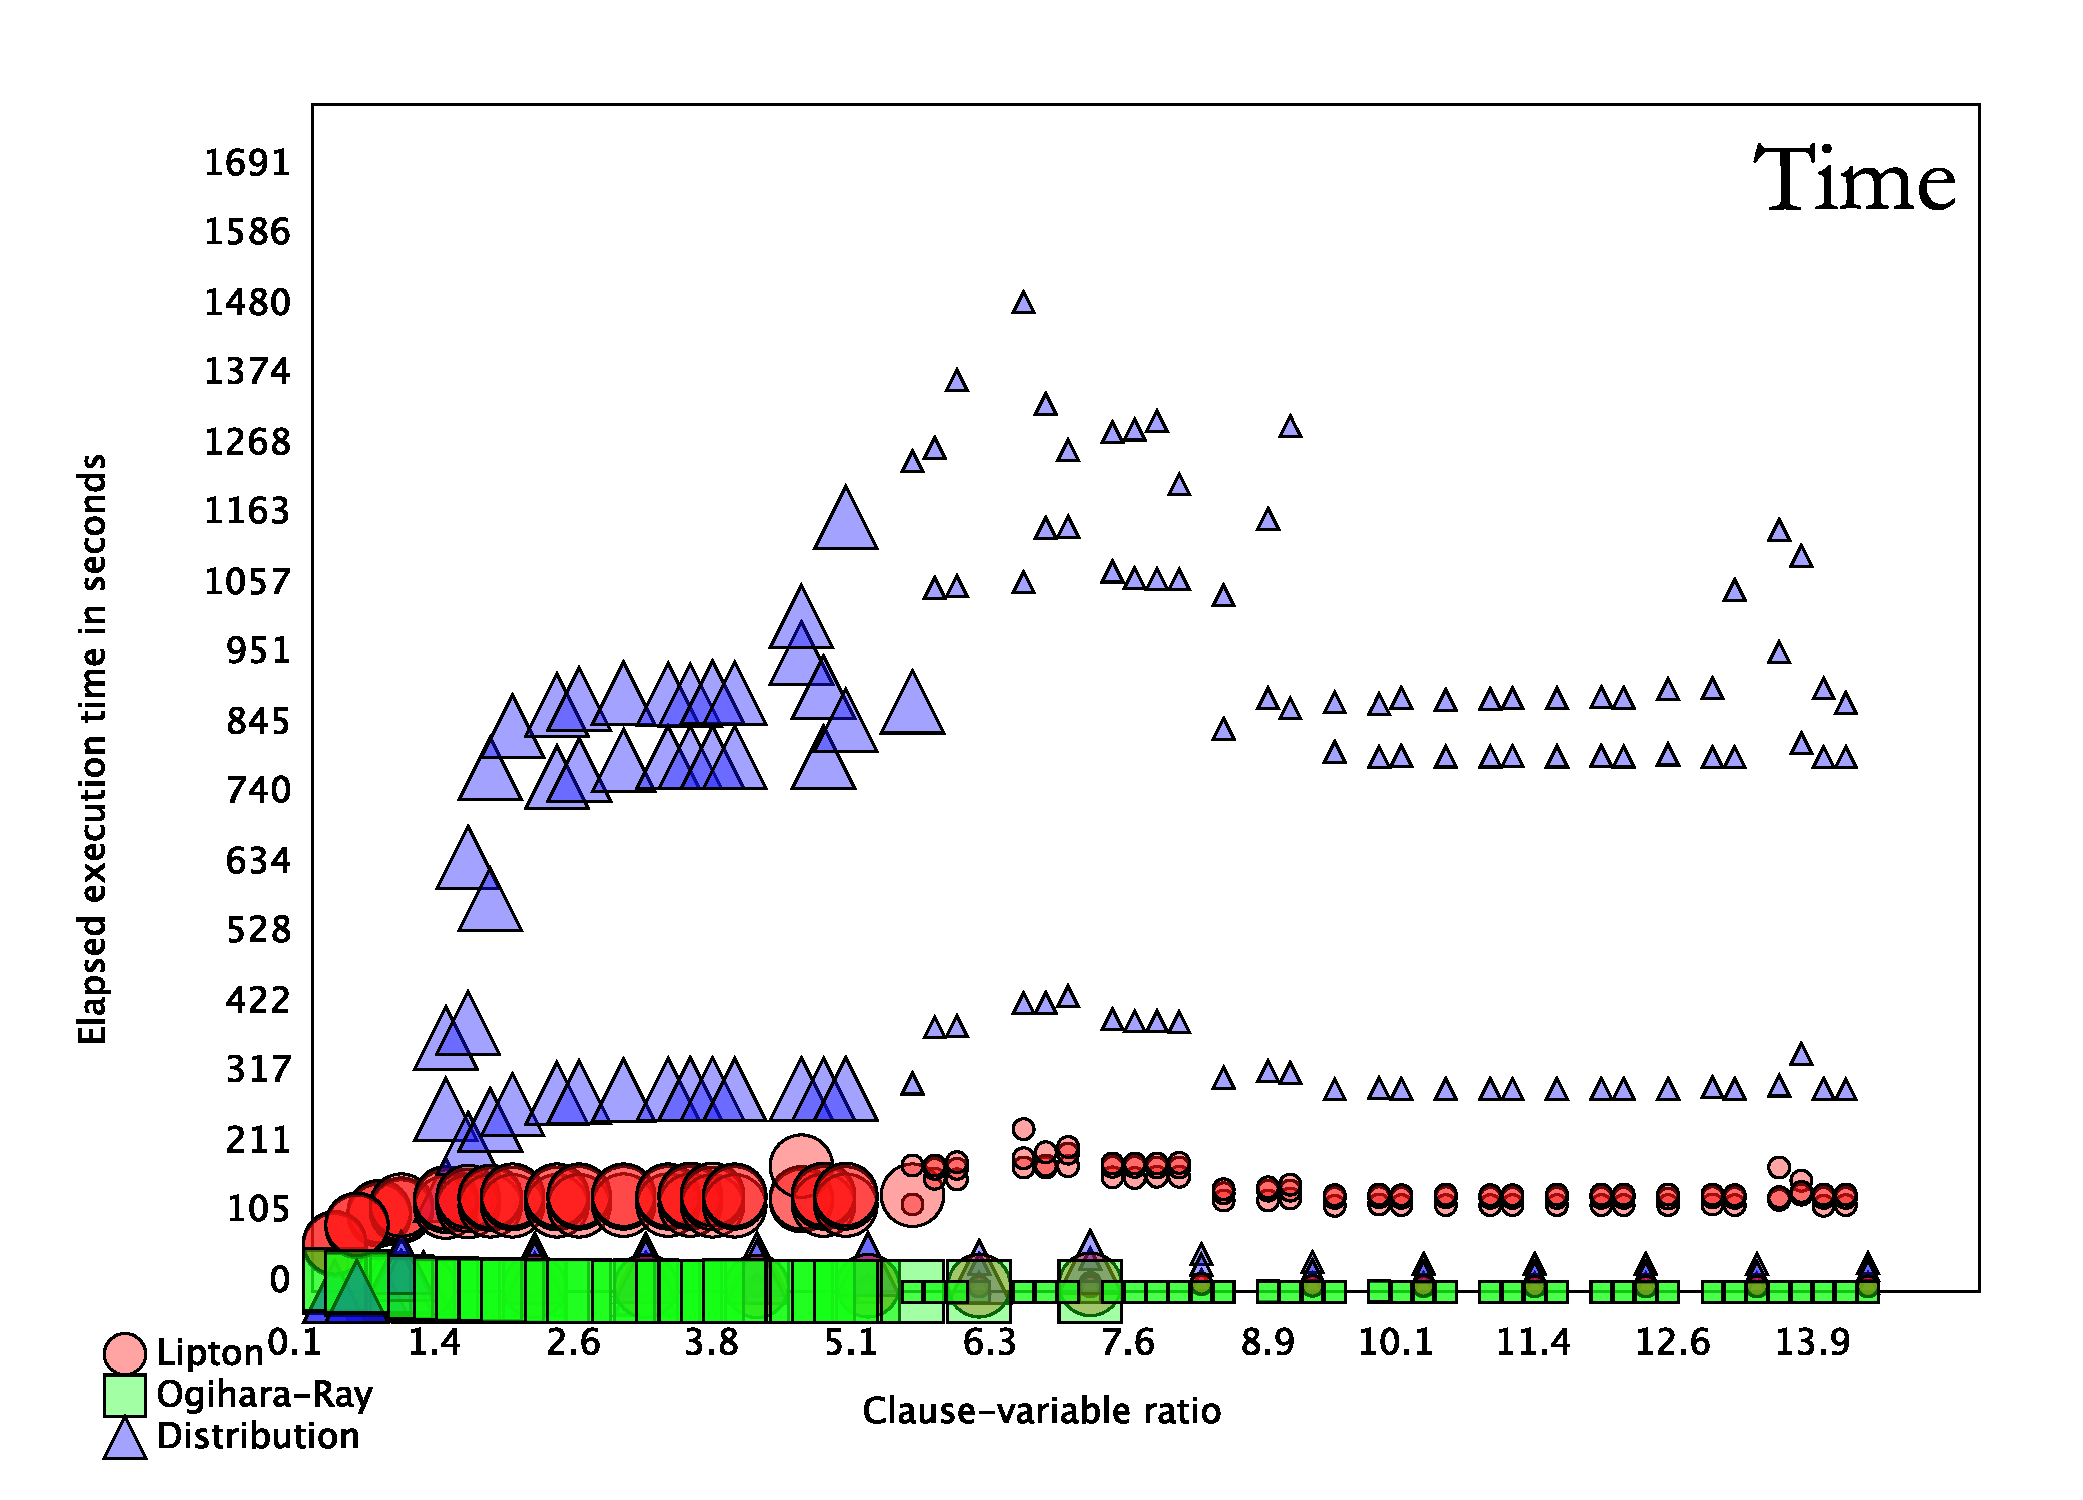
\includegraphics[width=1.1\textwidth]{./figures/metricOutput/Time.pdf}

\caption{Clause to variable ratio $\alpha$ vs. execution time in seconds }
\label{timeFig}
\end{center}
\end{figure}
%%%%%%%%%%%%%%%%%%%%%%%%%%%%%%%%%

\FloatBarrier
			
%\subsection{Solution space}
%%%%%%%%%%%%%%%%%%%%%%%%%%%%%%%%%
\begin{figure}[htdp]

\reversemarginpar{
\textbf{Memory} is a measurement of the satisfiable instance footprint returned by each algorithm measured in Bytes.\\

Lipton's and Ogihara-Ray's algorithms share the same solution footprint.

The Distribution algorithm contains a larger solution footprint after the trivially satisfiable instances with $\alpha \approx [0.2, 0.8]$.  The space provides a set of non-conflicting assignments from $\alpha \approx [0.8, 2.9]$.  Non-conflicting assignments consist of valuations for only necessary variables. \\

Each {\sc Satisfiability} instance has a constrained solution space during the phase-transition region.  All three algorithms share the same footprint.  There are no satisfiable instances in this test with $\alpha > 7.2$. The axis in Figure \ref{memoryFig} scales accordingly.
}


\begin{center}

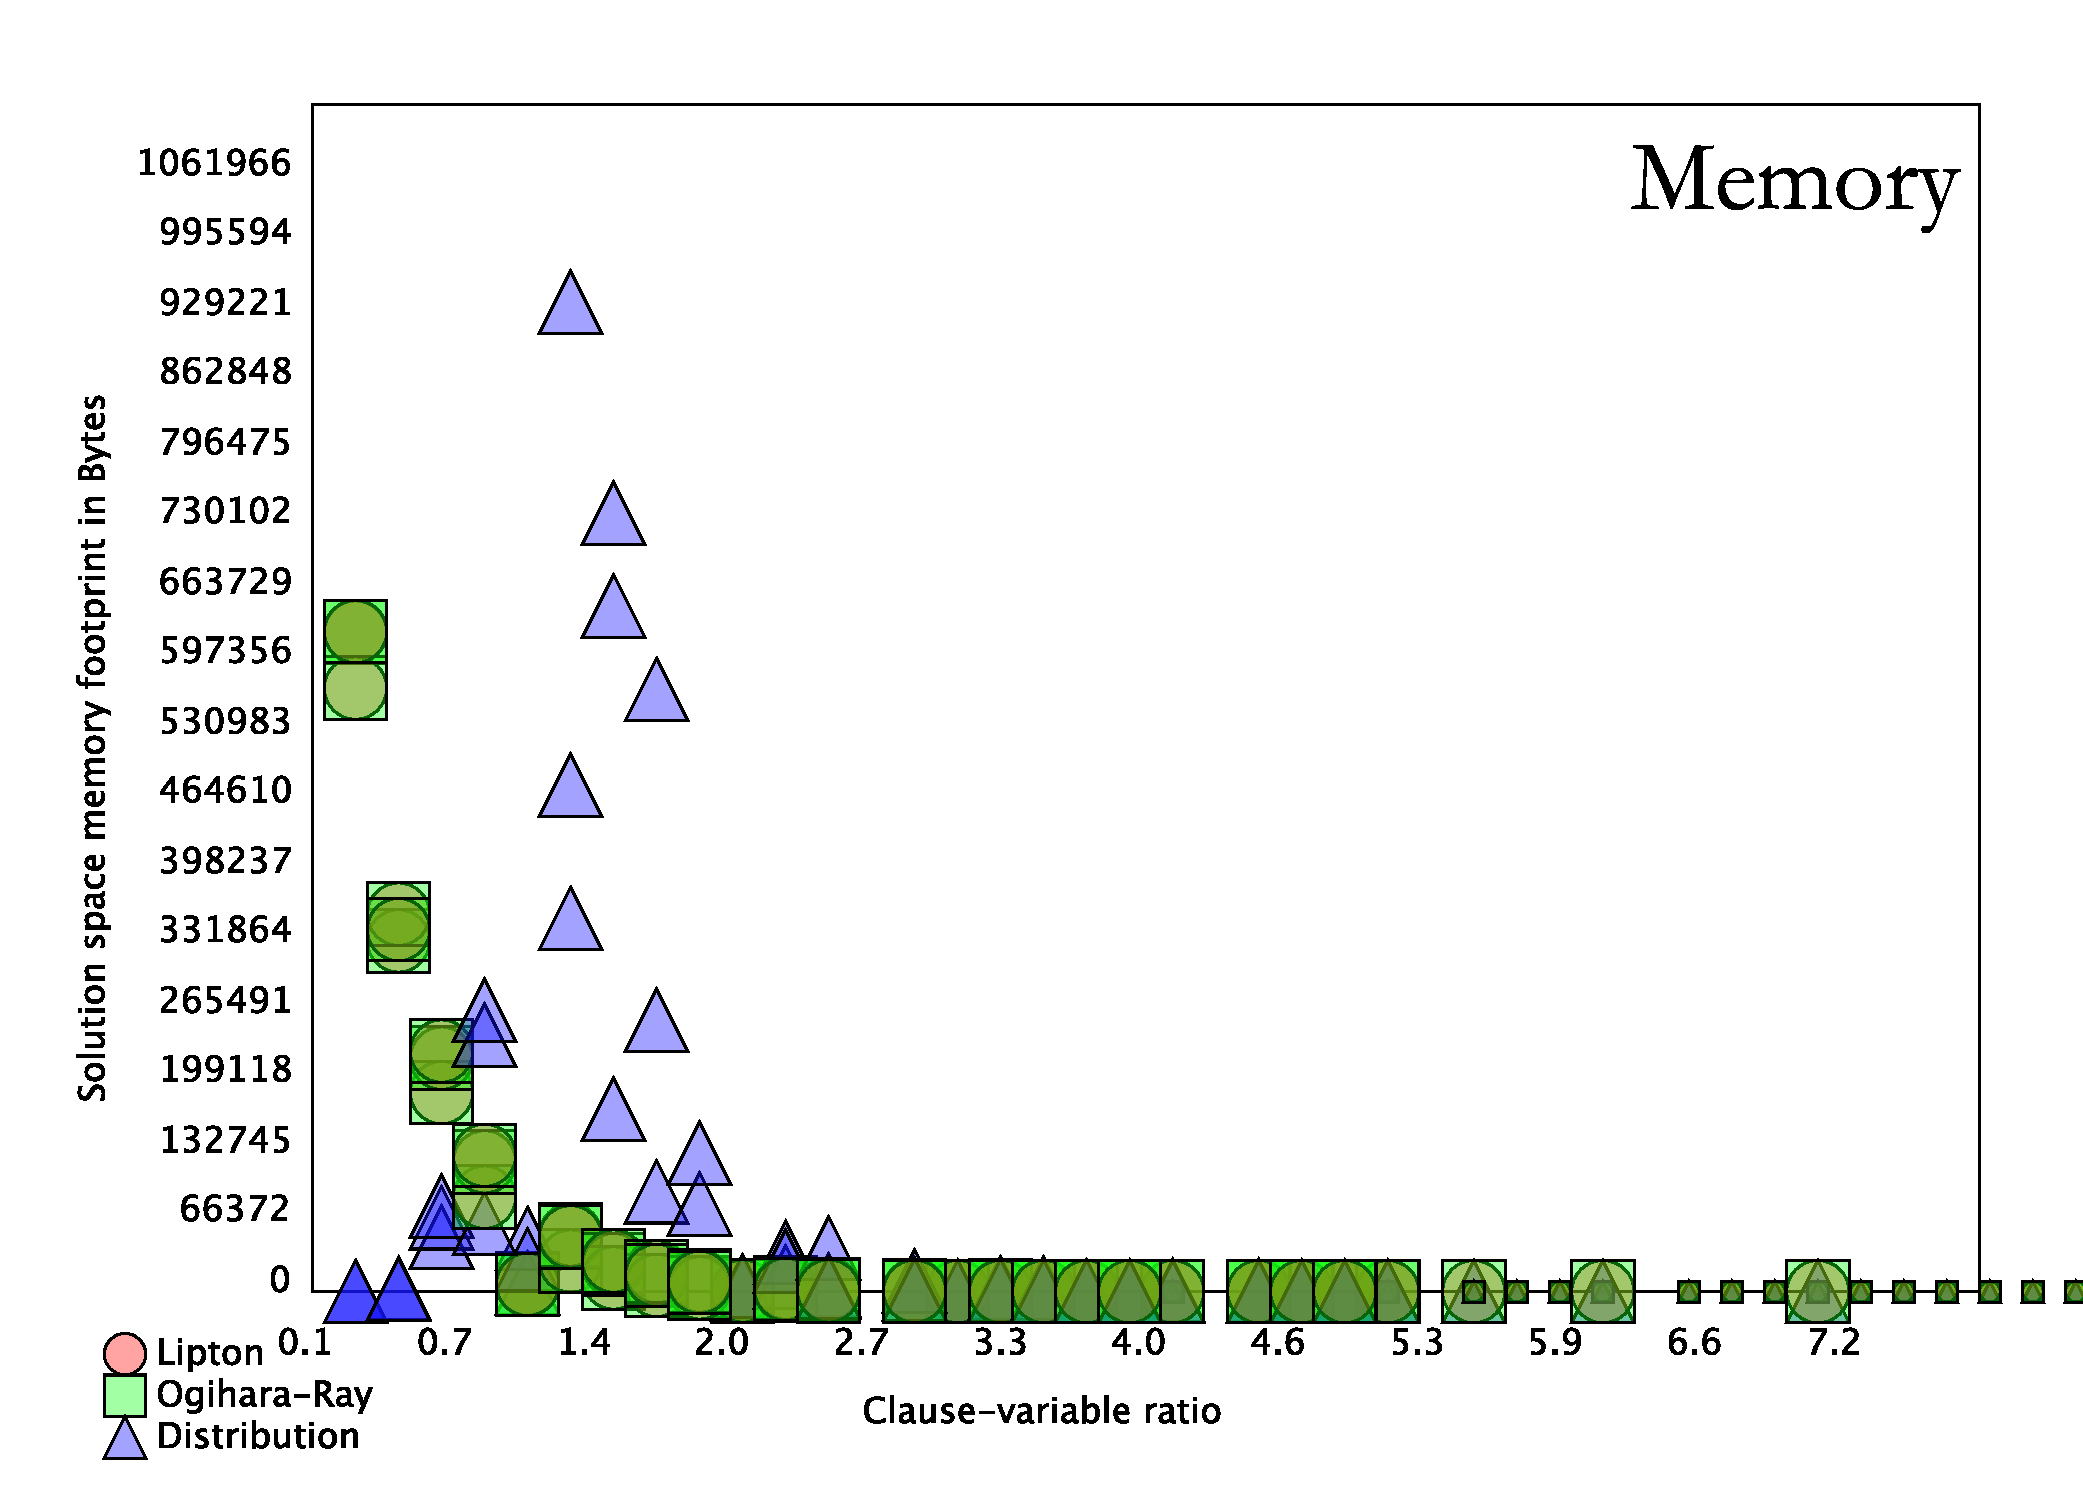
\includegraphics[width=1.1\textwidth]{./figures/metricOutput/Memory.pdf}

\caption{Clause to variable ratio $\alpha$ vs. satisfiable solution footprint in Bytes }
\label{memoryFig}
\end{center}
\end{figure}
%%%%%%%%%%%%%%%%%%%%%%%%%%%%%%%%%

\FloatBarrier


\section{On construction of a molecular computer}

%		<Paragraph> Describe outlook of techniques		

We consider present techniques in molecular biology and VLSI circuit construction as design considerations for a molecular computer.  We describe the selection of an encoding substrate and for sequence representation.  Implementation of the substrate considers properties from the molecular algorithms under test. 

%		<Paragraph> Describe how techniques may construct general computer

Continuing, we provide techniques for construction of a molecular computation environment.  The environment applies {\sc Satisfiability} as a standard algorithm for general computation.  This includes an execution pipeline for integration with existing silicon fabrication processes.
		
		\subsection{Selection of encoding substrate}
		
%			<Paragraph> Describe genetic encoding
During the introduction of molecular computation, we considered $+$DNA and $-$DNA as a computing substrate.  These choices were arbitrary to illustrate the automatic string matching mechanism of genetic information.  Physical implementations can use various substrates for artificial or practical significance.
			
%			<Paragraph> Understand consequences of molecular computing

Designing real molecules with artificial significance require consideration of the practical implications.  Physical features inadvertently encoded in a sequence may yield unexpected consequences.  This includes molecules with structural design flaws or potentially hazardous.
			
%			<Paragraph> Introduction to virology
%%%%Virology is the study of a type of hazardous molecules.  Virons are non-living molecules that require a host to operate.  Once active, the molecule interacts with a host cell to perform actions.  
			
%			<Paragraph> Constrained consequences of molecular computing

  Constraining molecular computation reduces the risk of external contamination.  We consider an environment constructed for isolation.  This eliminates external contamination of the molecular substrate and reduces the risk for contaminating the environment.

			
		\subsection{Selection of algorithm}
		
%			<Paragraph> Design of computing task
Molecular Simulation provides a simulation system for molecular {\sc Satisfiability} algorithms.  We have collected simulation results for a sweep of random $k$-{\sc Sat} instances.  Now we consider each of the algorithm's performance in terms of implementation in a physical system.
			
%			<Paragraph> Multiple considerations for general computation
We have seen that some of the metrics vary considerably.  Beneficial components of algorithm performance should be considered for physical implementation.  This includes the benefits of reducing an existing space versus construction of only possible combinations.
		
%			<Paragraph> Construction of a computational space
Construction of a computational space depends on the algorithm implementation.  Lipton's algorithm reduces a larger space to only the satisfiable solutions.  Ogihara and Ray's and the Distribution algorithm construct an incremental space based on the evaluation order.  The incremental construction decreases the total amount of required space for computing {\sc Satisfiability}.  With the Distribution algorithm, non-conflicting assignments provide shorter valuations without spanning all $n$ variables.
			
		\subsection{Selection of encoding mechanism}
		
%			<Paragraph> On virons and other molecular constructions
The encoding mechanism may exhibit features that can be utilized for desired functionality.  We consider construction and reuse of combinatorial spaces, along with permission of unbounded length restrictions.

%			<Paragraph> On combinatorial spaces
Lipton's algorithm begins with the construction of a combinatorial space. The algorithm discards the space after each {\sc Satisfiability} instance.  This does not need to be the case; the space can be recovered through a reaction process.  The process requires copying the discarded +DNA strands and from the satisfying solution.
			
%			<Paragraph> On unbounded length restrictions
Let us consider a molecular computer without a fixed length bound.  This machine is the same as the construction of a combinatorial space without regarding the a fixed number of variables.  With this machine, we can provide assertions for problems beyond a fixed problem instance.  Immediately we can represent much larger problems that are representable in the current vector space.  This leads to a possible security concern that may allow the user to increase the space for solving any problem.  The present oligonucleotide definition does not provide efficient encodings compared with natural genomes. 

			
		\subsection{Description of a self contained molecular computer}
		
%			<Paragraph> Overview
Manual laboratory procedures demonstrate molecular computation for single problem instances \cite{Adleman:1994:MCS:189441.189442, dnaBasedImplemetation_Yoshida2000, faulhammer2000mol, Braich02solutionof}.  These techniques are error prone due to human intervention.  Implementers have suggested robotic automation as a means to eliminate human contact \cite{dnaBasedImplemetation_Yoshida2000}.  However the techniques are an automated version of a human process.  We consider present gene sequencing technologies for the construction of a general molecular computer.
			
%			<Paragraph> Technology required
Integrated molecular computing technology gets inherited from sequencing technologies.  Nanopores provide a method for sequencing genetic sequences \cite{dnaTransistorIBMpressrelease, nanoporeChapter11, ionTorrent, oxfordNanopore}.  We apply nanopores along with integrated micropumps \cite{Liao_Lee_Liu_Hsieh_Luo_2005} for the transfer of molecules within an integrated architecture.     
			
%			<Paragraph> Construction techniques
Construction of the integrated architecture extends standard silicon processes.  A nanopore can be constructed by production of a silicon nitride ($\text{Si}_3\text{N}_4$) substrate and removing an hourglass shaped portion \cite{Heng_Aksimentiev_Ho_Marks_Grinkova_Sligar_Schulten_Timp_2006}.  Each side of the nanopore forms a membrane between two potentials \cite{Heng_Aksimentiev_Ho_Marks_Grinkova_Sligar_Schulten_Timp_2006}; the potential difference requires a concentration of potassium ($\text{K}^+$) and chlorine ($\text{C}^-$) ions in aqueous buffer solutions.  
	
%	<Figure>	Circuit description
\begin{figure}[htbp]
\begin{center}

	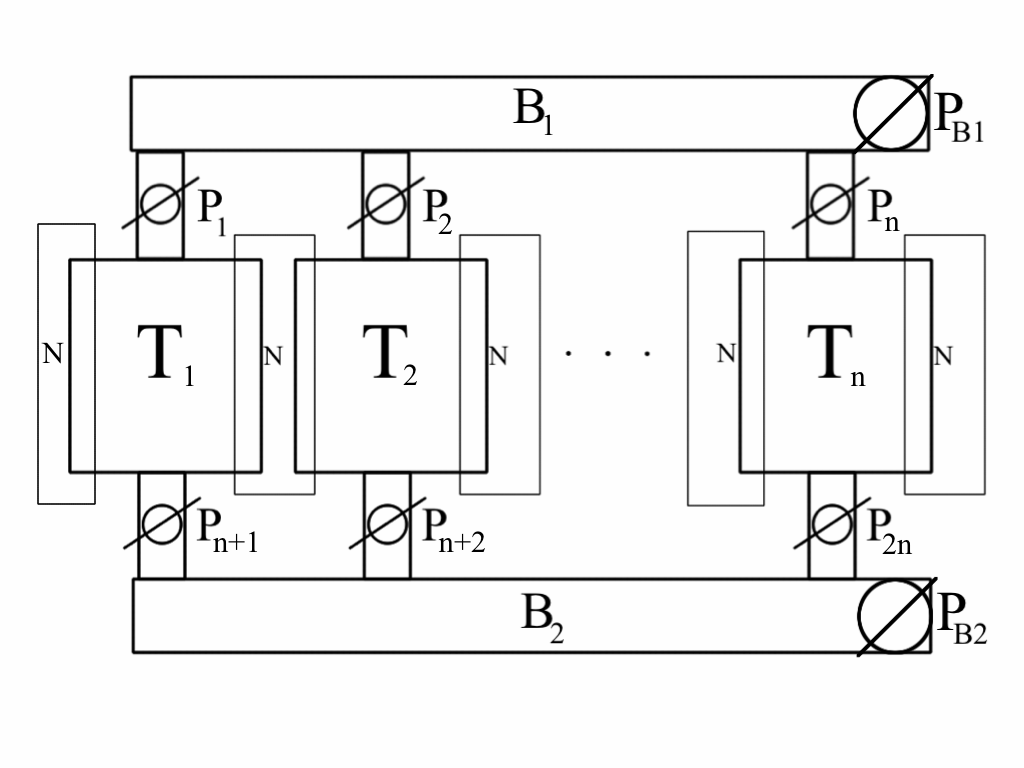
\includegraphics[width=0.7434\textwidth]{figures/molecularSchematic.png}

\caption{Schematic of molecular computing architecture.}
\label{molecularSchematic}
\end{center}
\end{figure}

\FloatBarrier	
	
Figure \ref{molecularSchematic} shows a schematic representation for a molecular computing architecture.  This architecture consists of a series of tubes connected with nanopores ($\text{N}$) and micropumps ($\text{P}$).  Each well ($\text{T}$) contain the representation of a test tube in a macro-experimental view.  Information between wells gets transfered through a stackable microtube data bus, labeled $B_1$ and $B_2$.  The microtube data bus provides transfer of buffer solution and preparation of wells.  

%			<Paragraph> Operating the machine
Control of the machine in Figure \ref{molecularSchematic} requires the transfer of buffer solutions along with molecular encodings between tubes.  Activating a micropump permits flow through the tube and directed movement of solutions through an internal configuration.  For example, directing the pumps $\text{P}_1$ and $\text{P}_{n+1}$ from $\text{B}_1$ to $\text{B}_2$ permit the contents of $\text{T}_1$ to be mixed with $\text{B}_2$.  Once this transfer occurs, then $\text{P}_{n+1}$ can be closed.  Subsequent operations may be performed with multiple tubes, and the contents directed to specified storage.  

%			<Paragraph> On reading and writing
Nanopores allow for reading and writing of genetic sequences.  In the molecular computing architecture the read and write cycle occurs in a isolated tube.  As a molecule passes through the nanopore, a current is induced according to the nucleotide present in the pore.  We cannot yet practically write molecules with nanopores.  Writing with nanopores requires modification of a molecular state, and can theoretically be accomplished \cite{dnaTransistorIBMpressrelease}.  The nanopore will consist of a full read-write component and provide an interface for external control.

%			<Paragraph> Interface with existing architectures 
Integration with existing computing architectures provides an interface to the user and a synergetic medium for general purpose computation.  Molecular computing can perform many tasks in parallel, however each operation may take orders of magnitude longer than conventional architectures.  For example, a conventional computer architecture may be used to verify valid configurations for {\sc Satisfiability} but cannot easily compute all valid configurations.  The computation of all configurations for a {\sc Satisfiability} problem instance may be executed as a combinatorial molecular process, and the solution written to a conventional computing medium.  This interface requires design and interaction with the user by leveraging the architecture as a dual computing environment.   
